% FILE: figures/catalytic_paths.tex
% Catalytic vs non-catalytic reaction paths

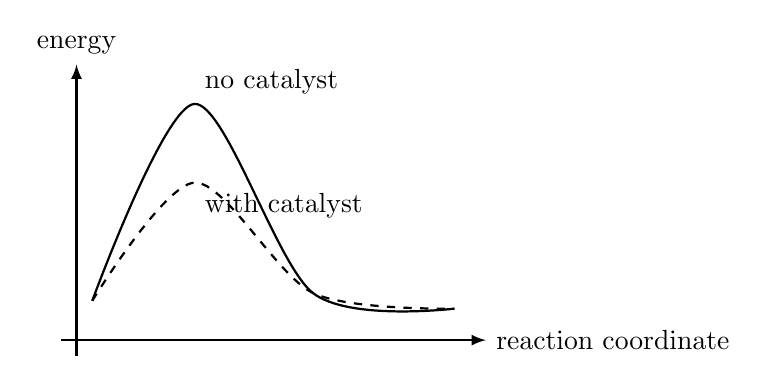
\begin{tikzpicture}[>=latex,thick,scale=1]
  % Axes
  \draw[->] (-0.2,0) -- (5.2,0) node[right] {reaction coordinate};
  \draw[->] (0,-0.2) -- (0,3.5) node[above] {energy};

  % Uncatalyzed path
  \draw[smooth,thick]
    plot coordinates {
      (0.2,0.5)
      (1.5,3.0)
      (3.0,0.6)
      (4.8,0.4)
    };
  \node[anchor=south west] at (1.5,3.0) {no catalyst};

  % Catalyzed path
  \draw[smooth,thick,dashed]
    plot coordinates {
      (0.2,0.5)
      (1.5,2.0)
      (3.0,0.6)
      (4.8,0.4)
    };
  \node[anchor=north west] at (1.5,2.0) {with catalyst};
\end{tikzpicture}

